%2.3.tex

ベクトル拡張付きRISC-Vは機械語コードが同時演算数に依存しないスケーラブルなベクトル拡張を実現したISAであり,ARM SVEを参考に仕様策定したものである.

従来のSIMD命令による処理ではSIMD演算器数の変更によって同時演算数を変化させることができるが,同時演算数の変更に伴って機械語コードの変更が必要である.例としてSIMD命令を用いて999個の要素を持つ配列同士の加算の処理を行う場合の同時演算数による違いを図\ref{fig:SIMD_ex}に示す.図\ref{fig:SIMD_ex}の(a)では同時演算数が2とした場合で(b)は同時演算数を4とした場合である.(a)では同時演算数が2であるためwhile命令によってSIMD演算を行った後に余りの要素を逐次処理によって処理を行っている.(b)では同時演算数を4に変更しており,同様にwhileによるSIMD演算を行った後に余りの要素の処理を行っているが,同時演算数を変更したことによって余りの要素の数が変わるため同時演算数が異なる場合機械語コードを作り直す必要がある.

\begin{figure}[tb]
    \centering
    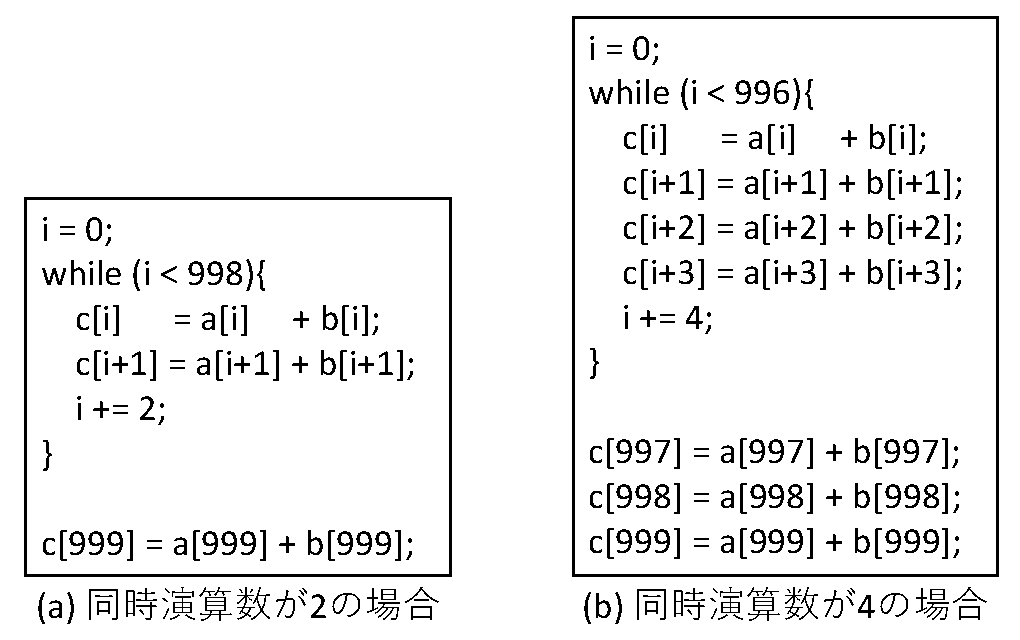
\includegraphics[scale=0.6]{image/SIMD_example.pdf}
    \caption{SIMD命令による配列加算の処理}
    \label{fig:SIMD_ex}
\end{figure}

対して,ベクトル拡張付きRISC-Vでは同時演算数に依存しないスケーラブルなベクトル拡張を行うためにプレディケートによるループ処理が行われる.ベクトル命令ではベクトルレジスタを用いた複数データの演算を行う際にプレディケートレジスタを用いたマスク処理が行われる.プレディケートレジスタではプレディケートレジスタの1ビットがベクトルレジスタの1要素の対応しており,プレディケートレジスタの値がTrueであるとき命令を実行し,Falseのときは命令を実行しないといった処理が行われる.
プレディケートレジスタを用いたループ処理を行うときに使う命令としてWHILE系命令がある.WHILE系命令では配列要素のベクトル演算を行う際にループカウンタと処理する配列の全要素数を比較してループカウンタが全要素数より小さい間対応するプレディケートレジスタの要素をTrueにする.ループカウンタが全要素数以上の場合,対応するプレディケートの要素をFalseにする.これによって余りの要素がある場合でもすべてのデータ数分ベクトル処理を行うことができ,同時演算数に依存しない機械語コードが実現できる.
WHILE系命令の例としてWHILELO命令の動作の概要を図\ref{fig:predicate}に示す.図\ref{fig:predicate}の(a)ではループカウンタがデータ数より小さい場合であり,プレディケートの要素が全てTrueになっている.図\ref{fig:predicate}の(b)では余りの要素の処理を行う場合であり,ループカウンタがデータ数より小さいときのみ要素がTrueとなっている.これによって余りの要素が変化した場合でも処理を行うことができる.

\begin{figure}[tb]
    \centering
    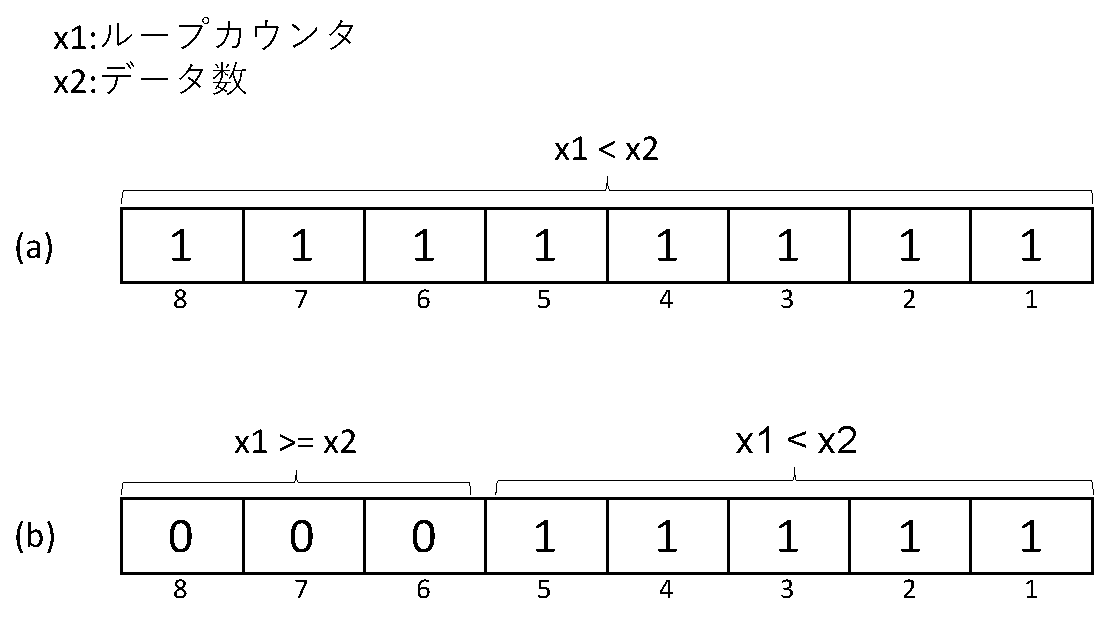
\includegraphics[scale=0.5]{image/predicate.pdf}
    \caption{WHILELO命令の動作}
    \label{fig:predicate}
\end{figure}

ベクトル拡張付きRISC-Vの命令体系を図\ref{fig:Inst_map}に示す.ベクトル拡張付きRISC-Vのベクトル命令はベクトルロード,ストア命令,ベクトル演算命令,ベクトル制御命令の3つに分けられる.RISC-Vにはカスタム命令用にオペコード領域が4つ用意されているがそのうちの2つを利用しており,1つをベクトルロード・ストア命令,もう一方をベクトル演算命令とベクトル制御命令に使用している.ベクトルロード・ストア命令のアドレスはベースとなるスカラレジスタの値にオフセットを加えることで計算する.
ベクトル演算命令は,プレディケートレジスタによるマスク処理を行うプレディケートあり演算命令,プレディケートレジスタによるマスク処理を行わないプレディケートなし演算命令,即値とベクトルレジスタによる演算を行う即値演算命令に分けられる.
ベクトル拡張付きRISC-Vは基本命令に関してRV32Iのみ組み込んでいる.

\begin{figure}[tb]
    \centering
    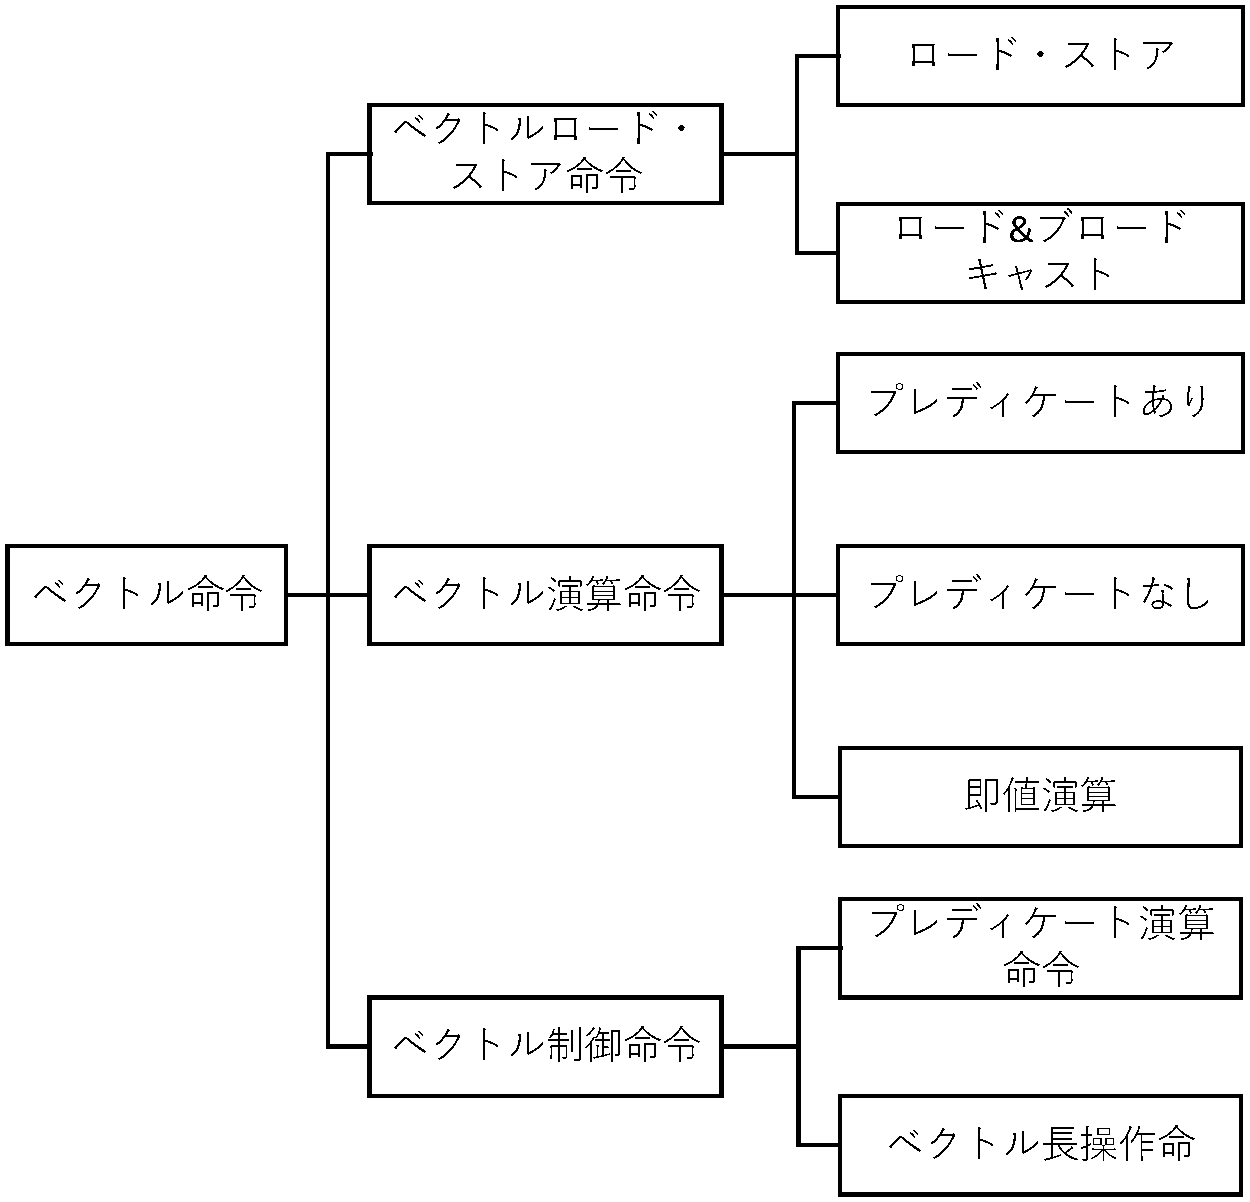
\includegraphics[scale=0.5]{image/Inst_map.pdf}
    \caption{ベクトル拡張付きRISC-Vの命令体系}
    \label{fig:Inst_map}
\end{figure}

レジスタ構成はベクトルレジスタv0-v31,ベクトルマスク制御に用いるためのプレディケートレジスタvp0-vp7,プレディケートレジスタ同士の論理演算に用いるプレディケートレジスタvp8-vp15,RISC-Vの汎用レジスタx0-x31,プログラムカウンタとなっている.ベクトルレジスタの長さは128$\times 2^n(0\leq n\leq 4)$ビットで表され,汎用レジスタの幅は32ビットとなっている.

ベクトル命令のフォーマットはRISC-Vの命令形式であるR形式に従ったものとなっている.また,デコーダの単純化のために同じフィールドにはできるだけ同じ機能をもたせている.

%図%図入れる
%にベクトル拡張付きRISC-Vのベクトル命令のフォーマットの一例を示す.命令はプレディケートありVADD命令,プレディケートなしVADD命令,即値によるベクトル加算命令であるVADDI,ロード,ストア命令であるVLW,VSW命令である.どの命令もデスティネーションレジスタを指定するためのフィールドは共通となっている.